\documentclass{tufte-handout}
% \documentclass{article}

%\date{28 March 2010} % without \date command, current date is supplied

% \geometry{showframe} % display margins for debugging page layout

\usepackage{graphicx} % allow embedded images
  \setkeys{Gin}{width=\linewidth,totalheight=\textheight,keepaspectratio}
  \graphicspath{{graphics/}} % set of paths to search for images
\usepackage{amsmath}  % extended mathematics
\usepackage{booktabs} % book-quality tables
\usepackage{units}    % non-stacked fractions and better unit spacing
\usepackage{multicol} % multiple column layout facilities
\usepackage{lipsum}   % filler text
\usepackage{fancyvrb} % extended verbatim environments
  \fvset{fontsize=\normalsize}% default font size for fancy-verbatim environments
\usepackage{listings}

% Standardize command font styles and environments
\newcommand{\doccmd}[1]{\texttt{\textbackslash#1}}% command name - - adds backslash automatically
\newcommand{\docopt}[1]{\ensuremath{\langle}\textrm{\textit{#1}}\ensuremath{\rangle}}% optional command argument
\newcommand{\docarg}[1]{\textrm{\textit{#1}}}% (required) command argument
\newcommand{\docenv}[1]{\textsf{#1}}% environment name
\newcommand{\docpkg}[1]{\texttt{#1}}% package name
\newcommand{\doccls}[1]{\texttt{#1}}% document class name
\newcommand{\docclsopt}[1]{\texttt{#1}}% document class option name
\newenvironment{docspec}{\begin{quote}\noindent}{\end{quote}}% command specification environment

\begin{document}

\title{MAE-253: Homework 3}
\author[John Karasinski]{John Karasinski}
\maketitle% this prints the handout title, author, and date

\section{Problem 1: Modularity matrix}

\section{1.1 Bisection of a binary undirected network}
\begin{figure}
  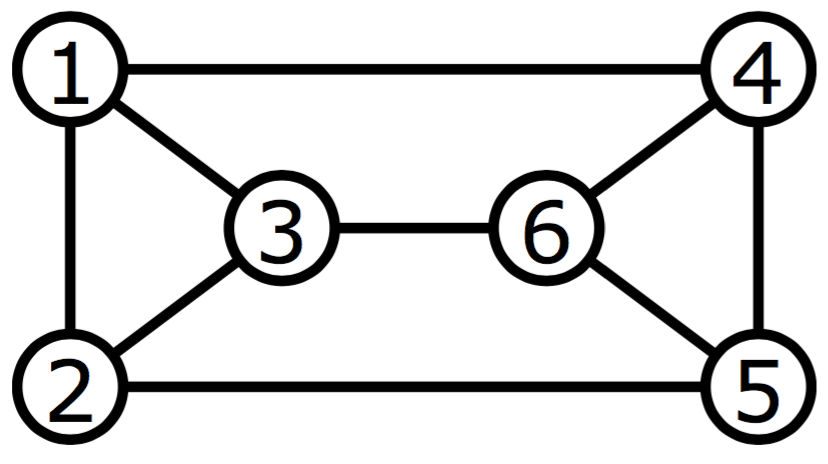
\includegraphics[width=0.5\linewidth]{1-1.png}
%  \checkparity This is an \pageparity\ page.%
  % \caption{This graph shows the community structure of the network. Each community is colored differently.
  % \emph{Notice that this figure only takes up the main textblock width.}
  % }
  \label{fig:textfig}
  %\zsavepos{pos:textfig}
  \setfloatalignment{b}
\end{figure}

\subsection{1. Consider the graph given above. Give the adjacency matrix ($A$) of this graph.}

\begin{align*}
A =
\begin{bmatrix}
  0 & 1 & 1 & 1 & 0 & 0 \\
  1 & 0 & 1 & 0 & 1 & 0 \\
  1 & 1 & 0 & 0 & 0 & 1 \\
  1 & 0 & 0 & 0 & 1 & 1 \\
  0 & 1 & 0 & 1 & 0 & 1 \\
  0 & 0 & 1 & 1 & 1 & 0
\end{bmatrix}
\end{align*}

\subsection{2. Let $m$ denote the total number of edges in this graph. Construct a matrix $B$ such that $B_{ij} =A_{ij} - \frac{k_ik_j}{2m}$.}

% A = pd.read_clipboard(header=None, delimiter='&', comment='\\').as_matrix()
% B = A - (A.sum(axis=0) * A.sum(axis=1))/(A.sum())

\begin{align*}
B =
\begin{bmatrix}
 -0.5 &  \phantom{-}0.5 &  \phantom{-}0.5 &  \phantom{-}0.5 & -0.5 & -0.5 \\
  \phantom{-}0.5 & -0.5 &  \phantom{-}0.5 & -0.5 &  \phantom{-}0.5 & -0.5 \\
  \phantom{-}0.5 &  \phantom{-}0.5 & -0.5 & -0.5 & -0.5 &  \phantom{-}0.5 \\
  \phantom{-}0.5 & -0.5 & -0.5 & -0.5 &  \phantom{-}0.5 &  \phantom{-}0.5 \\
 -0.5 &  \phantom{-}0.5 & -0.5 &  \phantom{-}0.5 & -0.5 &  \phantom{-}0.5 \\
 -0.5 & -0.5 &  \phantom{-}0.5 &  \phantom{-}0.5 &  \phantom{-}0.5 & -0.5
\end{bmatrix}
\end{align*}

\subsection{3. Obtain the eigenvalues of $B$ and list them.}
% np.linalg.eig(B)[0]

\begin{align*}
\lambda =
\begin{bmatrix} 1, -2, -2, 0, 0, 0
\end{bmatrix}
\end{align*}

\subsection{4. What is the eigenvector (say $v$) corresponding to the largest eigenvalue?}
% np.linalg.eig(B)[1][np.linalg.eig(B)[0].argmax()]

\begin{align*}
v(\lambda = 1) =
\begin{bmatrix} 0.408248, 0.408248, 0.408248, -0.408248, -0.408248, -0.408248
\end{bmatrix}
\end{align*}

\subsection{5. Look at the sign of each component of $v$. If $v_i > 0$ assign node $i$ to community 1 else assign node $i$ to community 2. List the nodes that belong to community 1 and nodes that belong to community 2. Is the assignment reasonable?}

\begin{align*}
c =
\begin{bmatrix} 1, 1, 1, 2, 2, 2
\end{bmatrix}
\end{align*}

Yes, this seems reasonable.

\subsection{6. Extra Credit: Why does this work?}

From Wikipedia, ``Modularity is the fraction of the edges that fall within the given groups minus the expected such fraction if edges were distributed at random.'' Our choice for assigning nodes to communities in 5. maximizes $Q = \frac{1}{2m} \sum_{ij} s_i B_{ij} s_j$, where $s$ is +1 for one community, and -1 for another community. In other words, we've chosen the groups that are the least likely to have randomly formed.

\section{1.2 Bisection of a weighted undirected network}
\begin{figure}
  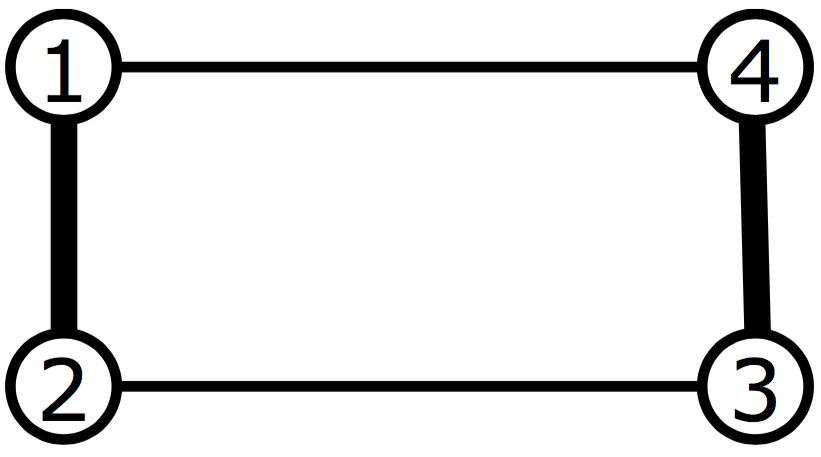
\includegraphics[width=0.5\linewidth]{1-2.png}
%  \checkparity This is an \pageparity\ page.%
  % \caption{This graph shows the community structure of the network. Each community is colored differently.
  % \emph{Notice that this figure only takes up the main textblock width.}
  % }
  \label{fig:textfig}
  %\zsavepos{pos:textfig}
  \setfloatalignment{b}
\end{figure}

\subsection{1. Consider the graph given above. Give the weighted adjacency matrix ($A$) of this graph.}

\begin{align*}
A =
\begin{bmatrix}
  0 & 5 & 0 & 1 \\
  5 & 0 & 1 & 0 \\
  0 & 1 & 0 & 5 \\
  1 & 0 & 5 & 0 \\
\end{bmatrix}
\end{align*}

\subsection{2. Let m denote the total weight of edges in this graph. You can obtain $m$ by summing all the entries in $A$ and dividing it by 2.}

\begin{align*}
m = 12
\end{align*}


\subsection{3. Construct a matrix B such that $B_{ij} =A_{ij} - \frac{k_ik_j}{2m}$.}

\begin{align*}
B =
\begin{bmatrix}
-1.5 & \phantom{-}3.5 & -1.5 & -0.5 \\
\phantom{-}3.5 & -1.5 & -0.5 & -1.5 \\
-1.5 & -0.5 & -1.5 & \phantom{-}3.5 \\
-0.5 & -1.5 & \phantom{-}3.5 & -1.5 \\
\end{bmatrix}
\end{align*}

\subsection{4. Obtain the eigenvalues of $B$ and list them.}
\begin{align*}
\lambda =
\begin{bmatrix} 4, 0, -6, -4
\end{bmatrix}
\end{align*}

\subsection{5. What is the eigenvector (say $v$) corresponding to the largest eigenvalue?}

\begin{align*}
v(\lambda = 4) =
\begin{bmatrix} 0.5,  0.5, -0.5, -0.5
\end{bmatrix}
\end{align*}

\subsection{6. Look at the sign of each component of $v$. If $v_i > 0$ assign node $i$ to community 1 else assign node $i$ to community 2. List the nodes that belong to each of the two communities? Is the assignment reasonable?}

\begin{align*}
c =
\begin{bmatrix} 1, 1, 2, 2
\end{bmatrix}
\end{align*}

This assignment is reasonable, as the nodes that are more highly linked are in communities.

\section{Problem 2: Pigou's congestion example}
Recall Pigou's example discussed in class, where there are two roads that connect a source, $s$, and destination, $t$. The roads have different travel costs. Fraction $x_1$ of the traffic flow on route 1, and the remainder $x_2$ on route 2. Here consider the following scenario.

\begin{itemize}
\item The first road has `infinite' capacity but is slow and requires 1 hour travel time, $T_1 = 1$.
\item The second road always requires at least 15 mins, which then increases as a function of traffic density, $T_2 = 0.25 + 0.75 x_2$.
\end{itemize}
If drivers act in a `selfish' manner - the user optimal scenario - all the traffic will flow on the second path, as one is never worse off. Worst case scenario for path 2, both paths take one hour. So no one is incentivized to change their behavior.
\subsection{1. Assume user optimal behavior, and calculate $\tau$ the expected travel time per car.}

\begin{align*}
\tau &= x_1 T_1 + x_2 T_2 \\
     &= x_1 (1) + x_2 (0.25 + 0.75 x_2) \\
     &= x_1 + 0.25 x_2 + 0.75 x_2^2 \\
\end{align*}
If $x_1 = 1 - x_2$, and $x_2 = x$, we have
\begin{align*}
\tau &= 1 - x  + 0.25x  + 0.75 x^2 \\
     &= 1 - 0.75x + 0.75 x^2 \\
\end{align*}

\subsection{2. If instead we could control the flows, we could minimize the expected travel time. Using the expression in part (a), calculate the optimal allocation of flows $\bar{x}_1$ and $\bar{x}_2$ that minimize the expected travel time per car.}

To minimize $\tau$ we take it's derivate and set it equal to zero,
\begin{align*}
0 &= - 0.75 + 1.5 x \\
x &= \dfrac{1}{3} \implies x_1 = \dfrac{2}{3}, x_2 = \dfrac{1}{3}\\
\end{align*}

\subsection{3. What is $\tau_m$, the expected travel time when the flow is optimized?}

\begin{align*}
\tau_m &= x_1 + 0.25 x_2 + 0.75 x_2^2 \\
&= \dfrac{2}{3} + 0.25 \left( \dfrac{1}{3} \right) + 0.75 \left( \dfrac{1}{3} \right)^2 \\
&= \dfrac{5}{6}
\end{align*}


\end{document}








